\documentclass[a4paper, 11pt]{article}
\usepackage[a4paper,left=2cm,right=2cm,top=1.8cm,bottom=2.8cm]{geometry}

%use English lang:
\usepackage[english]{babel}

\usepackage{pictex,amsmath,amsfonts,amssymb,amsthm,verbatim}
\usepackage{fullpage}
%\usepackage{algorithm,algorithmic}
\usepackage{gensymb}
\usepackage{mathrsfs}
\usepackage{hyperref}

\setlength{\voffset}{-0.25in}
\setlength{\headsep}{+0.5in}
\setlength{\parskip}{1em}
\setlength{\parindent}{0em}

\def\vu{\mathbf{u}}
\def\vv{\mathbf{v}}
\def\vb{\mathbf{b}}
\def\vw{\mathbf{w}}
\def\vs{\mathbf{s}}

%Bibliography
%\usepackage[backend = biber, style = authoryear]{biblatex}
%\addbibresource{HelloWorld.bib}
\usepackage{etoolbox}
\patchcmd{\thebibliography}{\section*{\refname}}{}{}{}

%Graphics packages:
\usepackage{graphicx, graphics}
\usepackage{tabularx, caption}
\usepackage{multirow, multicol}
\usepackage{setspace, tikz}
\usepackage{xcolor}
\usepackage{titlesec}
\usepackage{mdframed}
\usepackage{fancyhdr}
\usepackage{lastpage}
\usepackage[utf8]{inputenc}

%Box:
\newmdenv[linecolor=blue,
          skipabove=\topsep,
          skipbelow=\topsep,
          leftmargin=5pt,
          rightmargin=-5pt,
          innerleftmargin=5pt,
          innerrightmargin=5pt]{mybox}

%Minted (for code):
\usepackage{minted}
\newminted{C}{frame = lines, framerule = 2pt}
          
%Macro:
\newcommand{\quotes}[1]{``#1''}
\newcommand{\tf}{\textbf}
\newcommand{\ti}{\textit}
\newcommand{\ttt}{\texttt}
\newcommand{\ud}{\underline}
\newcommand{\rarrow}{\rightarrow}
\newcommand{\larrow}{\leftarrow}
\newcommand{\lrarrow}{\leftrightarrow}


%fancyhdr:
\setlength{\headheight}{40pt}
\pagestyle{fancy}
\fancyhead{} % clear all header fields
\fancyhead[L]{
    \begin{tabular}{rl}
        \begin{picture}(25, 15)(0, 0)
            \put(0, -8){
\includegraphics[width=8mm, height=8mm]{hcmut.png}}
        \end{picture}&
        \begin{tabular}{l}
            \textbf{\bf \ttfamily University of Technology, VNU-HCM}\\
            \textbf{\bf \ttfamily Faculty of Computer Science \& Engineering}
        \end{tabular} 	
    \end{tabular}
}

\fancyhead[R]{
    \begin{tabular}{l}
        \tiny \bf \\
        \tiny \bf
    \end{tabular}
}

\fancyfoot{} %clear all footer fields
\fancyfoot[L]{\scriptsize \ttfamily CC01 - Operating System}
\fancyfoot[R]{\scriptsize \ttfamily Page {\thepage}/ \pageref{LastPage}}
\renewcommand{\headrulewidth}{0.3pt}
\renewcommand{\footrulewidth}{0.3pt}

\begin{document}
    \begin{titlepage}
        \begin{center}
            HO CHI MINH CITY UNIVERSITY OF TECHNOLOGY, VNU HCM \\
            FACULTY OF COMPUTER SCIENCE AND ENGINEERING
        \end{center}

        \vspace{1cm}

        \begin{figure}[h!]
            \begin{center}
                
\includegraphics[width=3cm]{hcmut.png}
            \end{center}
        \end{figure}

        \vspace{1cm}

        \begin{center}
            \begin{tabular}{c}
                \multicolumn{1}{l}{\textbf{\LARGE OPERATING SYSTEM:}} \\
                ~~\\
                \hline
                \\
                \multicolumn{1}{l}{\LARGE Lab 8: Memory Allocation} \\
                \\
                \hline
                \\
                \hspace{5cm} Pham Minh Tuan - MSSV: 1752595
            \end{tabular}
        \end{center}
    \end{titlepage}

%New page:
\newpage

%Table of contents:
\renewcommand*\contentsname{Contents:}
\tableofcontents

%Newpage
\newpage

\section{Exercises}

\subsection{Questions: }

\begin{enumerate}
    \item Given six memory partitions of 300 KB, 600 KB, 350 KB, 200 KB, 750 KB, and 125 KB (in order), how would the first-fit, best-fit, and worst-fit algorithms place processes of size 115 KB, 500 KB, 358 KB, 200 KB, and 375 KB (in order)? Rank the algorithms in terms of memory utilization. \\
    
    \tf{Answer: } \\
    \begin{enumerate}
        \item First-Fit:
        \begin{itemize}
            \item 115KB is put into 300KB partition, the memory remaining is (185KB, 600KB, 350KB, 200KB, 750KB, and 125KB)
            \item 500KB is put into 600KB partition, the memory remaining is (185KB, 100KB, 350KB, 200KB, 750KB, and 125KB)
            \item 358KB is put into 750KB partition, the memory remaining is (185KB, 100KB, 350KB, 200KB, 392KB, and 125KB)
            \item 200KB is put into 350KB partition, the memory remaining is (185KB, 100KB, 150KB, 200KB, 392KB, and 125KB)
            \item 375KB is put into 392KB partition, the memory remaining is (185KB, 100KB, 150KB, 200KB, 17KB, and 125KB)
        \end{itemize}
        \item Best-Fit:
        \begin{itemize}
            \item 115KB is put into 125KB partition, the memory remaining is (300KB, 600KB, 350KB, 200KB, 750KB, and 10KB)
            \item 500KB is put into 600KB partition, the memory remaining is (300KB, 100KB, 350KB, 200KB, 750KB, and 10KB)
            \item 358KB is put into 750KB partition, the memory remaining is (300KB, 100KB, 350KB, 200KB, 392KB, and 10KB)
            \item 200KB is put into 200KB partition, the memory remaining is (300KB, 100KB, 350KB, 0KB, 392KB, and 10KB)
            \item 375KB is put into 392KB partition, the memory remaining is (300KB, 100KB, 350KB, 0KB, 17KB, and 10KB)
        \end{itemize}
        \item Worst-Fit:
        \begin{itemize}
            \item 115KB is put into 750KB partition, the memory remaining is (300KB, 600KB, 350KB, 200KB, 635KB, and 125KB)
            \item 500KB is put into 635KB partition, the memory remaining is (300KB, 600KB, 350KB, 200KB, 135KB, and 125KB)
            \item 358KB is put into 600KB partition, the memory remaining is (300KB, 242KB, 350KB, 200KB, 135KB, and 125KB)
            \item 200KB is put into 350KB partition, the memory remaining is (300KB, 242KB, 150KB, 200KB, 135KB, and 125KB)
            \item 375KB must wait since the remaining parition cannot be used to allocate for this process.
        \end{itemize}

        \item Rank the  3 algorithms:
        \begin{itemize}
            \item Of three algorithms used, the Best-Fit is the most efficient, then is the First-Fit and the last is Worst-Fit.
            \item Beside only the Worst-Fit algorithm is allowed to reject the request to be satisfied.
            \item Although the Best-Fit is the efficient algorithm, it take the time O(n) while the First-Fit is O(1).
        \end{itemize}
    \end{enumerate}
    \item  Compare the advantages as well as disadvantages of these allocation algorithms: First-Fit, Best-Fit, Worst-Fit. Use specific examples to support your answer.
    \begin{enumerate}
        \item First-Fit: 
        \begin{enumerate}
            \item Advantage: Less time required for allocation and deallocation, this is the fastest one of 3 algorithms.
            \item Disadvantage: External fragmentation.
        \end{enumerate}
            
        \item Best-Fit:
        \begin{enumerate}
            \item Advantage: Better memory utilization, only search for the suitable smallest memory partition.
            \item Disadvantage: This is algorithm is the slowest one to compare with the other two algorithms.  
        \end{enumerate}

        \item Worst-Fit:
        \begin{enumerate}
            \item Advantage: This algorithms works efficiently if the memory allocations are of the medium sizes partition.
            \item Disadvantage: External Fragmentation, waste memory blocks.
        \end{enumerate}
    \end{enumerate}
\end{enumerate}

\subsection{Programming Exercises: }

\par{This is what I gain so far for implement Best-Fit algorithm. Since the different between the Best-Fit and First-Fit algorithm is the blocks of memory it looks for, so I only change the way it look for the memory block in Best-Fit algorithm. The remaining in source code and the file main.c is the same after all.}

\bigbreak
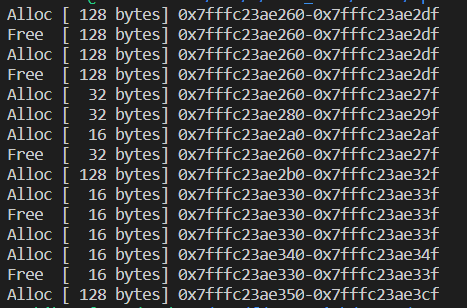
\includegraphics[scale = 0.7]{result.png}

\end{document}

%To compile this .tex file, you need to have -shell-escape in command to let the system understand the minted package: